\section{The evidence}\label{sec:crit-evidence}

\subsection{Fact 1, the anchor}

Fact~1 is the paper's strongest empirical asset: the only evidence that bears on a main result and could have failed. It sets the depletion of the frontier, the floor in the incidence theorem and the stepping-on-toes number. It is not yet at the standard its role requires.

\begin{enumerate}
\item \textbf{The baseline is taken at the wrong radius by the paper's own rule.} The text says that the model's topic is a cell of fixed size, ``so its density is the close-radius density. We therefore use $\EE=0.15$.'' But 0.15 is the middle of the \emph{broad}-radius range. At the close radius the estimate is 0.035 with a standard error of 0.118, an interval from $-0.20$ to $0.27$. The data reject a fixed idea space; they do not pin $\EE$.
\item \textbf{A less favourable estimate is omitted.} The project's own notes report 0.15--0.30 on the years before 2023. The full-sample 0.12--0.19 includes years in which the similarity measure drifted with the wording of abstracts. The paper uses this drift to withdraw its result on pioneering papers, but not to qualify Fact~1.
\item \textbf{The standard errors are the wrong ones.} They are clustered by author, while the regressor varies by area and year across 150 areas. The main range has no standard error at all.
\item \textbf{Attenuation is not discussed.} Only 58\% of a paper's nearest neighbours lie in its own area, which biases the estimate towards zero, the direction that favours the paper. The benchmark is built from the same noisy lists, which handles part of this; by one reader's calculation, 0.15 corresponds to roughly 0.19--0.28 once rescaled by the benchmark.
\item \textbf{Volume is not exogenous.} A new opportunity in an area raises its volume and lowers its local density at the same time. The paper concedes that the inversion ``assumes that the frontier did not move for other reasons''.
\item \textbf{It cannot be reproduced.} The panel behind Facts~1--4 is not in the repository and no script there produces them. The paper says that area clustering ``is part of the replication package''; the project's own notes list it as still open.
\end{enumerate}

The qualitative conclusion very probably survives: even 0.30 is well below 0.53. But the baseline, its interval and its reproducibility have to be repaired before anything is built on it. This is the first gate in Part~III.

\subsection{Fact 2 calibrates; it does not test}

Five of the eight calibration targets come from this one regression. Three points limit what it can carry.

First, ``density'' in the data is a paper's similarity to its nearest earlier papers, not the flow of a topic. Second, citations reward audience, which the paper acknowledges, so the gradient is an upper bound on the returns to density. Third, the one implication of the time-allocation margin that the data can see has the wrong sign. Run on the model's simulated data the way the regression is run on arXiv, papers per researcher fall by 1.3\% per standard deviation of density; in the data they rise by 0.5\% (standard error 0.1). The gap is about a quarter of the whole returns gradient. The paper calls it small.

\subsection{Facts 3 and 4: the credit block}

\begin{enumerate}
\item \textbf{A thin, selected tail.} The $-19\%$ and $+29\%$ compare 3,618 ``unaware'' and 1,381 ``aware'' flagged papers with 468,568 others. Whether a paper cites its nearest neighbour is correlated with its quality and with the prominence of the earlier paper.
\item \textbf{The correction for missed citations is applied to one fact and not the other.} The raw aware share among flagged papers is 27.6\%; corrected for the citations that PDF matching misses, it is about 60\% (Fact~4). So roughly 45\% of the papers called ``unaware'' in Fact~3 do cite the earlier paper. The $-19\%$ is the penalty of a mixed group, and the model's $\lambda$ is taken straight from it. If the misclassified papers earned the aware premium, the penalty for truly unaware duplicates would be far larger.
\item \textbf{At tight radii almost all close pairs share an author.} In high-energy physics the same-author share of later close pairs is 86\% at the 90th percentile of similarity and 95\% at the 99th. The ``other group'' tail on which the flag relies is small and sensitive to how authors are disambiguated.
\item \textbf{An assumed parameter.} The cost of pivoting (0.30) is an assumption, as is the distribution of follow-on credit.
\item \textbf{A contradiction.} Fact~3 says its estimate and the 21\% scooping penalty of Hill and Stein ``validate each other''. The model section says they ``measure different events'': one is duplication of earlier work, the other is losing a race.
\end{enumerate}

The damage is limited, because the main results do not depend on this block. That is also the argument for moving it out of the main text.

\subsection{``Adopters of language models produce 7\% more'' is a trend}

\begin{figure}[h]
\centering
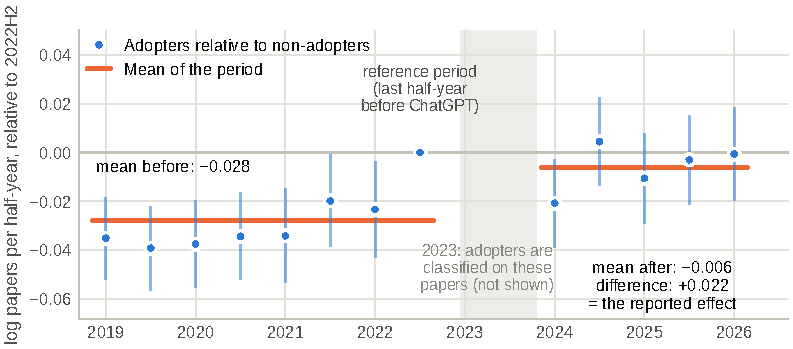
\includegraphics[width=\textwidth]{llm.pdf}
\caption{The paper's own event study, replotted from \texttt{empirics/results/llm\_authors.json}. Output of adopters relative to non-adopters, by half-year, with 95\% intervals; the last half-year before ChatGPT is the reference. The reported effect of 0.022 is the difference between the two orange lines. Relative to the reference period the effect after adoption is zero.}
\label{fig:llm}
\end{figure}

The estimate of 0.022 log points compares the average after 2023 with the average before. But adopters were already catching up with non-adopters before ChatGPT existed: the coefficients rise from $-0.035$ in 2019 to $-0.02$ in 2022. Relative to the last half-year before ChatGPT, the five coefficients after adoption average $-0.006$. A linear trend fitted to the earlier coefficients predicts $+0.010$ for the later window, so against trend the effect is about $-0.016$. The paper says that ``part of this is a pre-existing trend''. All of it is.

The classification is also noisy. Marker words appear in 3.0\% of abstracts in 2022 and 6.6\% in 2023, and 93\% of adopters are classified on one or two flagged abstracts. Adopters already used these words in 6.1\% of their abstracts in 2021--22, against 2.5\% for non-adopters.

This matters in three places: the introduction sets the 7\% against the 36\% of another study; Fact~5 rests on it; and Appendix~B.8 uses it to bound the size of the production shock ``so far'' at ``a few percent''.

\subsection{The designs, one by one}

\begin{center}\small
\begin{tabularx}{\textwidth}{@{}P{1.0in}L@{}}
\toprule
Design & What the review found \\
\midrule
\textbf{Endorsement rule} & The outcome is who presses ``submit''. Re-run on \emph{authors}: in Mathematics the share of papers with a first-time author does not fall ($-0.005$, standard error 0.004, on a base of 0.18), and the staggered contrast is zero ($-0.002$, 0.005). Outside Mathematics new authors per paper fall by about 14\%, with no control group and in the months of the 2026 surge. The paper's sentence that ``the entry margin responds to its cost, which is what makes density respond little to volume'' confuses entry into science with the supply of new topics. The prediction attached to it has no power: the model predicts a change in density of 0.5\% against a minimum detectable effect of two thirds of the base. \\
\textbf{Review rule} & A strong, well-timed first stage ($-1.3$ points, robust to a trend, no leakage). The reduced form on first-time authors ($-0.70$) has a placebo nearly half its size ($-0.32$); the difference is $-0.38$ with a standard error of about 0.31. It is not mechanical ($-0.72$ excluding review-titled papers), but it has no power in counts. The reviews removed are those not accepted by peer review, and reviews still appear after acceptance, so the rule delays more than it removes. Reviews are identified by words in titles, which the rule gives authors a reason to drop. Nothing shows that newcomers used the reviews that disappeared. ``Halved'' describes the share; the count fell by 35\%. \\
\textbf{Listing rank} & A clean design. But its first stage is not significant ($-0.023$ log citations per log position, standard error 0.016), and there are no data on downloads. A zero effect on later overlap is what one would see if detection worked through targeted search, and also if reading did not protect at all. The outcome measures related work, not duplicates. And in the model detection never depends on how prominent the earlier paper was. ``Tight bounds'' and ``detected by targeted search, not by browsing'' go beyond a joint null. \\
\textbf{Submission cap} & No object in the model, as the paper says. The cross-category dose--response is $+0.03$ with a standard error of 2.95, where mechanical removal would give $-1$: it has no content. Fifteen days of data. The sentence that a binding cap ``would be largely dissipated by entry'' contradicts Corollary~2: a cap binds on explorers too and would pass through at about 0.99. \\
\textbf{Daily cutoff} & Correctly discarded by the authors. \\
\bottomrule
\end{tabularx}
\end{center}

\subsection{The fact the paper misses: output per author jumped in 2026}\label{sec:surge}

\begin{figure}[h]
\centering
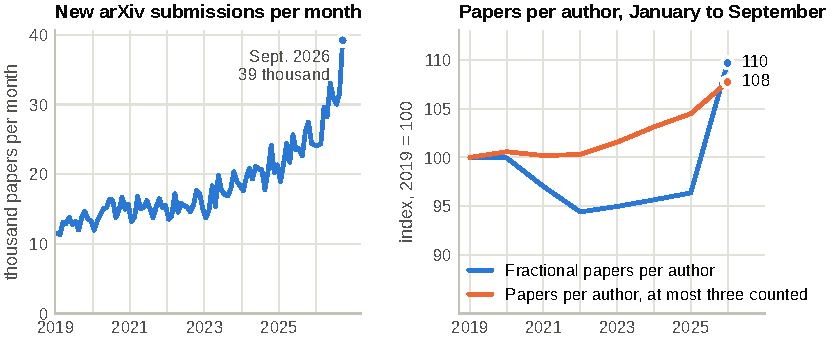
\includegraphics[width=\textwidth]{surge.pdf}
\caption{Computed from \texttt{data/arxiv\_meta.parquet}. Left: new submissions per month. Right: papers per author in January--September of each year, for names with full first names on papers with at most 30 authors. ``Fractional'' gives each author $1/n$ of a paper with $n$ authors.}
\label{fig:surge}
\end{figure}

The paper says that papers per author ``stayed flat'', that growth ``came mostly from new authors'', and that the rise in production so far is ``at most a few percent, too small to produce a visible spike in overlap or to close any topic''. The first two statements are true through 2025. The third is contradicted by the data in the repository.

\begin{center}\small
\begin{tabularx}{\textwidth}{@{}Lrr@{}}
\toprule
January--September & 2025 & 2026 \\
\midrule
Papers & 208,127 & 271,220 ($+30\%$) \\
Papers per submitter (1.47--1.53 in every year 2019--2025) & 1.53 & 1.69 \\
Fractional papers per author (0.50--0.53 in every year 2019--2025) & 0.508 & 0.578 ($+14\%$) \\
\quad the same, authors already active before & 0.580 & 0.658 \\
\quad the same, rare surnames only & 0.444 & 0.497 \\
\quad the same, a fixed cohort active in 2022--24 & 0.556 & 0.634 \\
Share of papers with one author & 10.8\% & 14.8\% \\
Mathematics, papers in September & 3,849 & 8,167 \\
\bottomrule
\end{tabularx}
\end{center}

After seven flat years, output per author rose by 11--14\% in nine months. The rise holds for established authors, for rare names and for fixed cohorts, so it is not a change in who is counted. Of the 30\% growth in volume, between 39\% and 49\% is output per person.

Three cautions belong with the fact.

\begin{itemize}
\item \textbf{It is concentrated among prolific names.} Counting at most three papers per name, the rise is 3.1\% (against 1.3\% the year before); uncapped it is 8.9\% in whole papers. Common names that pool several people inflate this tail.
\item \textbf{It is still building.} Papers per submitter were about 2\% above the previous year in January and February and 6.5\% above in September.
\item \textbf{It is not a pure shock to speed.} The number of authors also rose by about 15\%, three rule changes fall in the same months, and nothing shows what the extra papers are worth.
\end{itemize}

\begin{ideabox}[Why this matters more than any other finding]
Fact~1 was estimated on 2018--2025, years in which output per author was flat. It therefore measures how science absorbs \emph{more researchers}. The paper then uses it to speak about \emph{faster researchers}, which is an extrapolation. The year 2026 is the first time volume grew through output per author. The model says the two kinds of growth land in different places, and for once the data to check a headline claim are already on disk. Part~III builds the recommended paper on this.
\end{ideabox}

\subsection{First data on whether founders stay}

The founders' share is the missing statistic of the incidence theorem. A first cut from data on disk (high-energy physics, 2017--2022) shows that it can be measured, and that the measurement is not straightforward.

Of the later papers that land close to a given paper within two years, 65--70\% share an author with it at a moderate similarity threshold, and 86--96\% at tight ones. But most of this is authors continuing work that nobody else joined. Of 2,476 papers with at least three later close neighbours, 1,046 have no outside author among them. Where at least one outsider follows, the original authors write about 39\% of the later papers; where three or more outsiders follow, about 12\%.

So the founders' share is probably not zero and probably not one half. It is a share of \emph{value}, not of papers; the window is two years; and the radius is a choice. A proper measurement takes two to three weeks (\S\ref{sec:tests}).

\subsection{Statements left over from the previous version}

Eleven statements in the evidence sections contradict the current theory or point to the wrong place. The substantive ones are the ``validate each other'' sentence, the ``faster drafting'' prediction attributed to a proposition about production speed, the cap ``dissipated by entry'', and the attribution of the low volume elasticity to the cost of entering science. The full list is in Appendix~\ref{sec:app-errors}.
